\section{Multi-Robot Approach for Weld Cost Minimization}

In the approach section(cite section) we discussed how introduction of another robot can increase the number of degrees of freedom and hence allow the robot to perform more complex manipulations. Increasing the degree of complexity of motion can allow us to implement better optimization as well as solve the problems of unreachability and singularity. In this chapter we will discuss the integration of a 2 degrees of freedom rotary table into the existing architecture and how that is utilized to optimize the welding task. 

\subsection{Modeling the Rotary Table}
The existing implementation only contained kinematic description of the 6 axis manipulator with the weld tool tip. In the following subsections, we present a model of the 2 degree of freedom rotary table, along with the kinematic description and present the improved architectural model.
\subsubsection{Architecture of RobotKit}
The following architectural diagram(\ref{fig:img9}) has been color coded for better understanding. Blue represents the core functionalities of RobotKit. Red represents the kinematics and visualization models on which the improvements are implemented. Green represents external configuration files that are loaded inside RobotKit. Yellow represents the OMPL based planning library and pink represents the user interface block. \\
In the existing architecture the Kernel block creates instances of the kinematics and visualization models of the 6 Dof robot, which update the simulation environment based on the data input from the Information Exchange Pipeline. The planner interface class takes input from the kernel and the information exchange pipeline and user input for welding task. It then creates a planning problem and sends it to the OMPL based planning library. The communication between the planner interface and the planning library takes place using dll files. The project configuration file loads information about the dH parameters of the robot, position of the work piece and other relevant objects and in the weld cell. 

\begin{figure}[!htbp] %  figure placement: here, top, bottom, or page
 \centering
   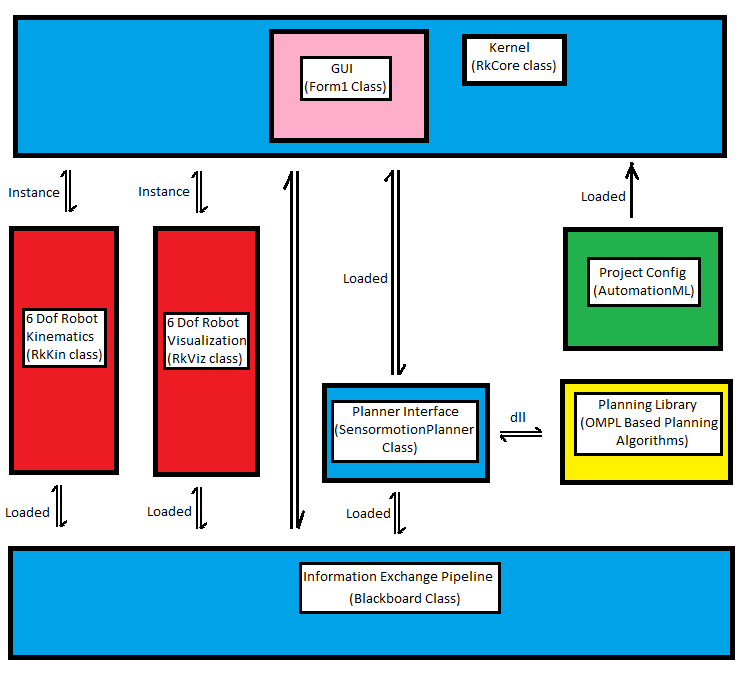
\includegraphics[width=9cm]{images/Original_arch.png}
   \caption[Exisitng Architecture of RobotKit(cite rk)]
   {Exisitng Architecture of RobotKit}  
\label{fig:img9}
\end{figure}

In the following architecture diagram (\ref{fig:img10}) the exact blocks which have been updated are highlighted. The kinematic and the visualization models now also includes definition of rotary table. The project configuration file (highlighted in green) has also been updated to include the dH parameters of the rotary table. 
\begin{figure}[!htbp] %  figure placement: here, top, bottom, or page
 \centering
   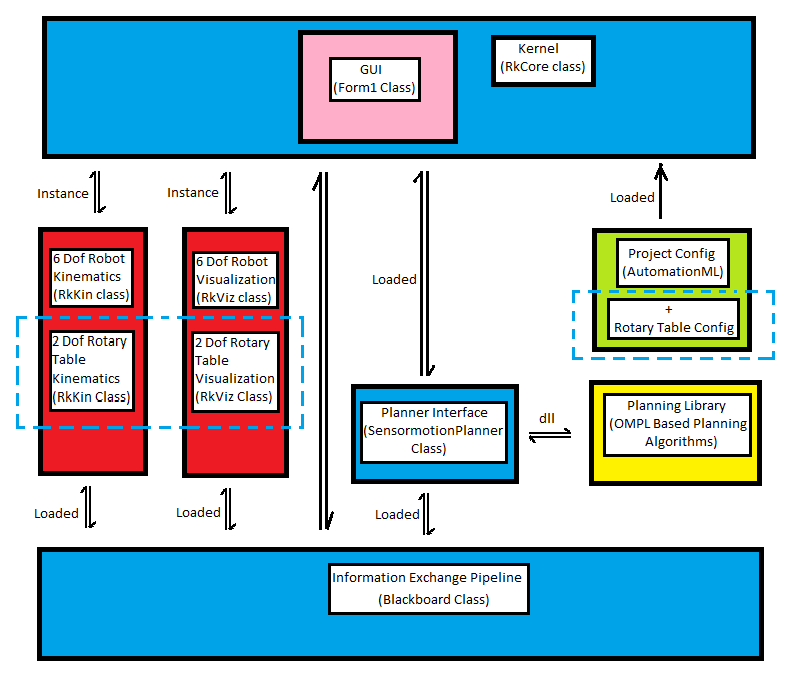
\includegraphics[width=9cm]{images/new_arch.png}
   \caption[Updated Architecture of RobotKit(cite rk)]
   {Updated Architecture of RobotKit}  
\label{fig:img10}
\end{figure}
 

\subsubsection{Generating 3D Models for Simulation}
In order to update the simulation environment, 3D CAD models of the rotary table were created using Solidworks software(cite solidworks), based on the data-sheet specifications. In order to make the simulation mimic the real functioning of the rotary table, the table was divided into 3 separate CAD objects; base, middle joint and top plate. The images for the same are presented herewith. 

\begin{figure}[!htbp] %  figure placement: here, top, bottom, or page
\begin{subfigure}{\linewidth}
   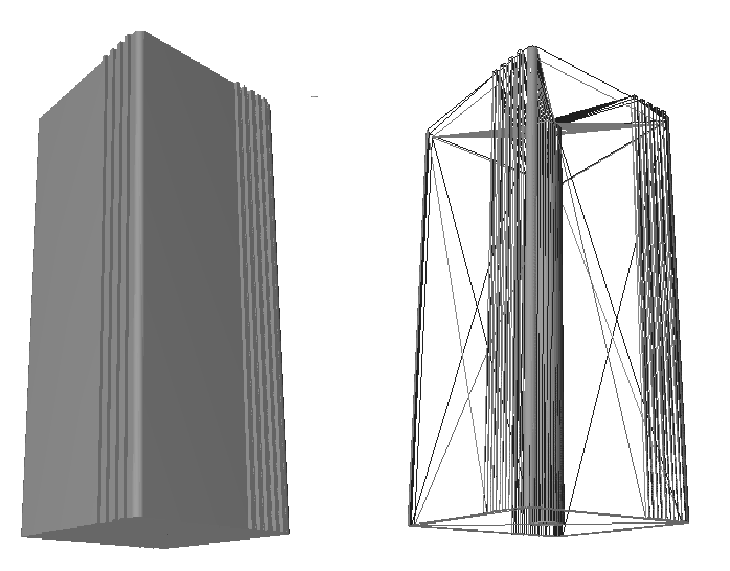
\includegraphics[width=.5\linewidth]{images/Base.png}
   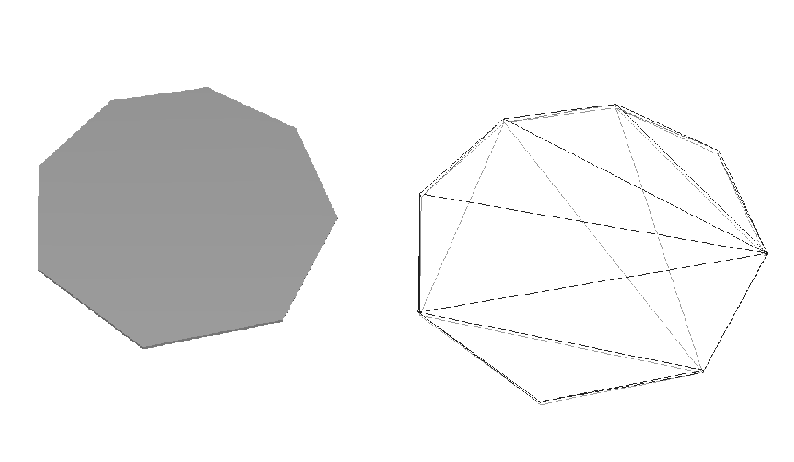
\includegraphics[width=.5\linewidth]{images/Top.png}
      \caption[dd]{Base and Top Joint models}
   \end{subfigure}\par\medskip
   \begin{subfigure}{\linewidth}
   \centering
   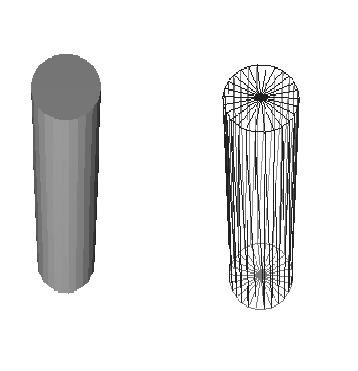
\includegraphics[width=.5\linewidth]{images/Mid.png}
   \caption[dd]{Middle Joint model}
   \end{subfigure}
\caption[dd]{CAD models of the Rotary Table: Base, Middle and Top}
\label{fig:img11}
\end{figure}
 

\subsubsection{Kinematic Description of the Rotary Table}
\subsubsection{Workpiece Transformation}
\subsubsection{Selected Edge Transformation}
